\documentclass[aps,prb,twocolumn,nofootinbib,superscriptaddress,floatfix]{revtex4-2}

\usepackage{amsmath,amssymb,amsthm,mathtools,bm}
\usepackage{booktabs}
\usepackage{graphicx}
\usepackage[colorlinks=true,linkcolor=blue,citecolor=blue,urlcolor=blue]{hyperref}
\usepackage{microtype}

\hypersetup{
  pdftitle={Bipartite mutual information of flattened domain-wall ground states},
  pdfauthor={Class-A fermionic adaptive-circuit project},
  pdflang={en-US},
  pdfdisplaydoctitle=true
}

\graphicspath{{figures/}}

\newcommand{\Tr}{\operatorname{Tr}}
\newcommand{\dd}{\mathrm{d}}
\newcommand{\cfit}{c_{\mathrm{fit}}}
\newcommand{\Iab}{I_{a,b}}
\newcommand{\Hflat}{\hat H_{\mathrm{flat}}}
\newcommand{\hflat}{h_{\mathrm{flat}}}

% Inline full-width material in the two-column grid.  RevTeX double-column
% floats can insert empty spacer pages when several full-page figures are
% forced in sequence; this environment uses the class's own grid switch and
% keeps each result figure on exactly one explicit page.
\makeatletter
\newenvironment{wideblock}{%
  \par\ignorespaces
  \setbox\widetext@top\vbox{%
    \hb@xt@\hsize{\hfil\vrule\@width\z@\@height2\p@}%
  }%
  \setbox\widetext@bot\hb@xt@\hsize{%
    \vrule\@width\z@\@depth2\p@\hfil
  }%
  \onecolumngrid
  \vskip2\p@
  \dimen@\ht\widetext@top\advance\dimen@\dp\widetext@top
  \cleaders\box\widetext@top\vskip\dimen@
  \vskip1\p@
  \prep@math@patch
  \noindent\begin{minipage}{\textwidth}
}{%
  \end{minipage}
  \par
  \vskip1\p@
  \setbox\widetext@bot\vbox{%
    \hb@xt@\hsize{\hfil\box\widetext@bot}%
  }%
  \dimen@\ht\widetext@bot\advance\dimen@\dp\widetext@bot
  \cleaders\box\widetext@bot\vskip\dimen@
  \vskip2\p@
  \twocolumngrid\global\@ignoretrue
  \@endpetrue
}
\newenvironment{widefigure}{%
  \begin{wideblock}\def\@captype{figure}\centering\vspace*{0.18in}
}{%
  \end{wideblock}
}
\makeatother

\begin{document}

\title{Bipartite mutual information of flattened domain-wall ground states}
\author{Internal campaign summary}
\affiliation{Class-A fermionic adaptive-circuit project}
\date{September 4, 2026}

\begin{abstract}
We compute deterministic reference curves for the half-filled ground state of
the overcomplete-Wannier flattened parent associated with a class-A adaptive
Chern circuit.  The spatial geometry is a periodic $N_x\times N_y$ torus
with $N_x=20$, two domain walls, and two opposite full-$x$ strips of width
$w=\lfloor N_y/4\rfloor$.  For $N_y=20,24,28$ at
$n_{\mathrm{shell}}=1$, and for $N_y=40,50,60$ at
$n_{\mathrm{shell}}=1,2,\infty$, we evaluate the strip mutual information and
the finite-size entropy slope for hard support-truncated and soft untruncated
wall constructions across a 21-point sweep from $\alpha_1=3$ to $1$.  In the
topological regime the mutual information approaches the free-Dirac
fixed-cross-ratio value $(\log 2)/3=0.2310491$ for exact quarter strips, while
the entropy slope gives $\cfit\simeq1$.  The mutual information does not
diverge under this finite-size scaling because strip width and separation grow
in the same proportion, leaving the conformal cross-ratio fixed.  The
full-frame enhancement just below $\alpha_1=2$ lies in a bulk-critical
finite-size window, but it does not coincide with the smallest saved
half-filling gap; it is not evidence for a stable wall theory with central
charge greater than one.  These
results are exact-Hamiltonian benchmarks, not results of the planned
Born-trajectory dynamical sweep.
\end{abstract}

\maketitle
\setcounter{tocdepth}{2}
\tableofcontents

\section{Scope and principal conclusions}
\label{sec:scope}

The class-A adaptive protocol of Bhuiyan, Pan, and Jian (BPJ) constructs
localized, nonorthogonal overcomplete Wannier (OW) modes from a two-band Chern
parent and uses their occupation measurements as a local controller
\cite{BhuiyanPanJian2026}.  A spatially patterned controller creates two
parallel domain walls on a periodic system.  The purpose of the calculation
reported here is deliberately narrower than a simulation of that circuit: we
form the quadratic OW flattened parent, fill its lowest half of single-particle
levels, and measure entanglement in the resulting Slater determinant.  There
are consequently no Born outcomes, stochastic trajectories, time evolution,
or sampling error bars in this note.

Three conclusions survive changes in circumference and wall construction.
First, in the topological regime the opposite-strip mutual information tends
to the free-Dirac value at the chosen cross-ratio, while the single-strip
entropy has a logarithmic coefficient consistent with one nonchiral Dirac
channel.  Second, shortening the OW support displaces and broadens the
finite-size crossover relative to the untruncated parent transition at
$\alpha_1=2$.  Third, the sharp enhancement of the full-frame estimators just
below $\alpha_1=2$ occurs where the bulk correlation length contaminates a
wall-only fit.  The saved half-filling diagnostics do not support attributing
that enhancement to a zero-mode degeneracy, and it must be separated from the
stable $\cfit\simeq1$ plateau at smaller $\alpha_1$.

All entropies and mutual informations below use natural logarithms and are
therefore measured in nats.  The production arrays, CSV tables, and their
checksum-bound completion records remain the authoritative numerical
products; the figures in this note are a read-only rendering of those arrays.

\section{Flattened OW parent and domain walls}
\label{sec:model}

\subsection{Uniform parent and OW frame}

The auxiliary Bloch Hamiltonian is the two-band matrix
\begin{align}
 h_{\alpha}(\bm k)
 &=\widehat{\bm n}_{\alpha}(\bm k)\cdot\bm\sigma,
 \\
 \bm n_{\alpha}(\bm k)
 &=\bigl(\sin k_x,\sin k_y,
 \alpha-\cos k_x-\cos k_y\bigr),
 \label{eq:bloch}
\end{align}
Away from a band closing, the spectral projectors are
$P_{\pm}(\bm k)=[\mathbf{1}\pm h_{\alpha}(\bm k)]/2$.
Projecting two trial orbitals
$\tau_{\nu}$, $\nu=A,B$, into the two bands and Fourier transforming produces
the OW states $\lvert W_{\bm r,\nu,\pm}\rangle$.  They are normalized after
the real-space support and wall masks are applied, but they are neither
orthogonal nor a linearly independent Wannier basis.  Their frame matrices are
\begin{equation}
 F_{\pm}=\sum_{\bm r,\nu=A,B}
 \lvert \widetilde W_{\bm r,\nu,\pm}\rangle
 \langle \widetilde W_{\bm r,\nu,\pm}\rvert.
 \label{eq:frame}
\end{equation}
The single-particle matrix and number-conserving many-body Hamiltonian used in
this benchmark are
\begin{align}
 \hflat&=F_+-F_-,
 \\
 \Hflat&=\sum_{i,j}\hat c_i^\dagger
 (\hflat)_{ij}\hat c_j.
 \label{eq:hflat}
\end{align}
Here ``flattened'' refers to the signs assigned to the upper- and lower-band
OW frame contributions.  Because the OW frame is overcomplete, $\hflat$ need
not itself have only the eigenvalues $\pm1$.

For each configuration we diagonalize $\hflat$ and occupy its lowest
$N/2=N_xN_y$ single-particle eigenvectors, where $N=2N_xN_y$ includes both
orbitals.  If $V_{\mathrm{occ}}$ denotes the matrix of occupied vectors, the
ground-state correlation projector is
\begin{equation}
 C=V_{\mathrm{occ}}V_{\mathrm{occ}}^\dagger,
 \qquad C^2=C=C^\dagger.
 \label{eq:projector}
\end{equation}

\subsection{Hard and soft interfaces}

The fixed transverse size is $N_x=20$.  The topological controller occupies
$x=5,\ldots,15$ and uses $\alpha_1$; the exterior uses
$\alpha_2=30$.  Thus the two interfaces are at $x=5$ and $x=16$, as shown in
Fig.~\ref{fig:geometry}.  For the hard wall, an OW mode is multiplied by a
domain mask that forbids its support from crossing either interface before
the mode is normalized.  For the soft wall, this additional mask is absent:
the parent parameter is still selected by the mode center, but the resulting
mode may extend across an interface.  The shell mask restricts periodic
coordinate differences to at most $n_{\mathrm{shell}}$ cells in each
direction; $n_{\mathrm{shell}}=\infty$ retains the full OW mode.

\begin{figure*}[t]
  \centering
  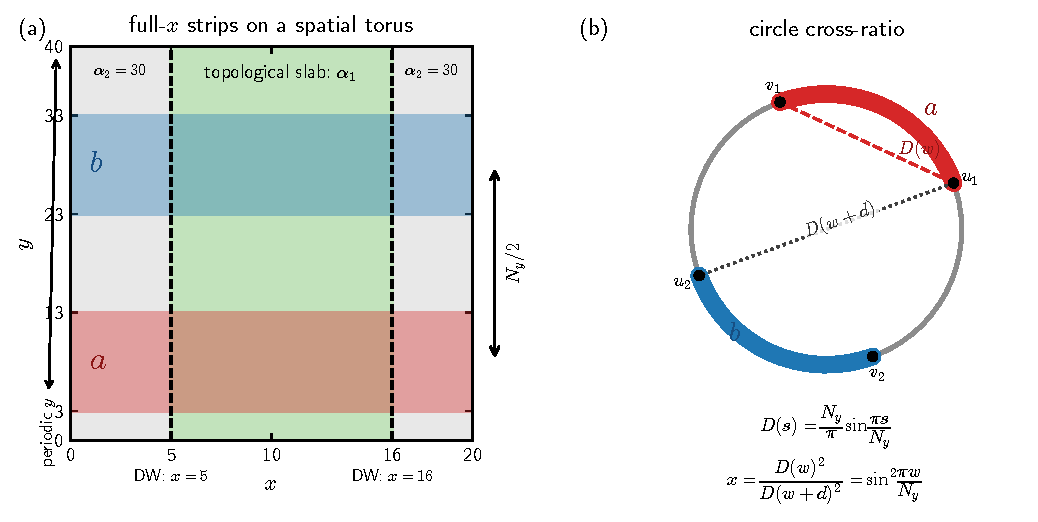
\includegraphics[width=0.98\textwidth]{geometry_and_cross_ratio.pdf}
  \caption{\label{fig:geometry}
  Mutual-information geometry and its one-dimensional CFT reduction.
  (a) The full-$x$ regions $a$ and $b$ include both orbitals and cross both
  domain walls.  Their starting points differ by $N_y/2$ on the periodic
  $y$ circle.  The drawing uses the representative $N_x=20$, $N_y=40$ case;
  $a$ and $b$ each have width $w=N_y/4=10$.  The topological slab comprises
  sites $x=5,\ldots,15$, so its interfaces lie at $x=5$ and $x=16$.
  (b) The wall degrees of freedom see two equal intervals on a circle.
  Conformal mapping replaces a line distance $s$ by its chord distance
  $D(s)=(N_y/\pi)\sin(\pi s/N_y)$.  For opposite intervals,
  $w+d=N_y/2$, and the cross-ratio reduces to
  $x=D(w)^2/D(w+d)^2=\sin^2(\pi w/N_y)$.}
\end{figure*}

\subsection{Campaign matrix and deterministic solver}

Table~\ref{tab:campaign} summarizes the two completed CPU calculations.  Both
use complex128 arithmetic, exact half filling, the $X$ trial-orbital pair,
and the same descending $\alpha_1$ grid,
\begin{multline}
 \{3,2.75,2.5,2.3,2.2,2.15,2.1,2.075,2.05,2.025,2,
 \\
 1.975,1.95,1.925,1.9,1.85,1.8,1.7,1.5,1.25,1\}.
 \label{eq:alphagrid}
\end{multline}
The first campaign performs dense Torch diagonalization.  The second exploits
exact translation symmetry along $y$: Fourier transformation reduces
$\hflat$ to $N_y$ independent blocks of dimension $2N_x=40$, which are
diagonalized with NumPy/SciPy.  Filling the lowest half of the combined block
spectrum is equivalent to diagonalizing the full matrix.

\begin{table*}[t]
\caption{\label{tab:campaign}
Deterministic flattened-ground-state campaigns.  Each listed point is one
Hamiltonian ground state rather than an ensemble of trajectories.}
\begin{ruledtabular}
\begin{tabular}{lcccccc}
campaign & $N_x$ & $N_y$ & $w$ & $n_{\mathrm{shell}}$ & walls & cases \\
\hline
small circumference & 20 & $20,24,28$ & $5,6,7$ & $1$ & hard, soft & 126 \\
large circumference & 20 & $40,50,60$ & $10,12,15$ & $1,2,\infty$ & hard, soft & 378
\end{tabular}
\end{ruledtabular}
\end{table*}

\subsection{Critical-grid prescription}

The allowed periodic momentum grid contains $\bm k=\bm0$.  At the uniform
parent transition $\alpha=2$, Eq.~\eqref{eq:bloch} gives
$\bm n_{2}(\bm0)=\bm0$, so $\widehat{\bm n}_{2}(\bm0)$ and the upper/lower
band decomposition are not uniquely defined.  The completed implementation
uses the symmetric numerical prescription
\begin{equation}
 h_{2}(\bm0)=0,
 \qquad P_+(\bm0)=P_-(\bm0)=\frac{\mathbf{1}}{2}.
 \label{eq:criticalprescription}
\end{equation}
The two matrices in Eq.~\eqref{eq:criticalprescription} resolve the identity
but are not idempotent spectral projectors.  Accordingly, every plotted
$\alpha_1=2$ point is a finite-grid midpoint convention, not either one-sided
limit of the gapped band projector.  Open markers identify those points in the
result figures.  Plateau and crossover claims are based on the neighboring
gapped values rather than on the precise midpoint value.

\section{Gaussian entropy and estimators}
\label{sec:estimators}

For a number-conserving Gaussian state, the reduced density matrix of a region
$R$ is fixed by the restricted correlation matrix $C_R$.  If its eigenvalues
are $\lambda_q\in[0,1]$, the von Neumann entropy is
\begin{equation}
 S_R=-\Tr\left[C_R\log C_R+
 (\mathbf{1}_R-C_R)\log(\mathbf{1}_R-C_R)\right],
 \label{eq:gaussianentropy}
\end{equation}
which is evaluated by diagonalizing $C_R$ \cite{Peschel2003,PeschelEisler2009}.
Numerically, eigenvalues are clipped only inside the logarithm at
$10^{-12}$; the unclipped extrema are retained as diagnostics.

For every allowed translation $y_0$, define
\begin{align}
 a(y_0)&=[0,N_x)\times[y_0,y_0+w),
 \\
 b(y_0)&=[0,N_x)\times
 [y_0+N_y/2,y_0+N_y/2+w),
 \label{eq:strips}
\end{align}
with periodic $y$ wrapping and both orbitals included.  The nonlinear
observable is formed before translation averaging,
\begin{equation}
 \Iab(y_0)=S_{a(y_0)}+S_{b(y_0)}-S_{a(y_0)\cup b(y_0)}.
 \label{eq:mi}
\end{equation}
The small-size campaign explicitly averages Eq.~\eqref{eq:mi} over
$N_y/2$ placements; the omitted half exchanges $a$ and $b$.  Its largest
spread over $y_0$ is $2.74\times10^{-12}$.  The large-size solver uses exact
$y$-translation symmetry to evaluate one placement and verifies a shift by
one lattice row, for which all recorded entropy and mutual-information
differences vanish at saved precision.

The single-strip entropy profile uses widths
$A_y=1,\ldots,N_y/2$.  We determine an operational central-charge estimator
from the unweighted fit
\begin{align}
 S(A_y)&=m\log\left[
 \frac{N_y}{\pi}\sin\left(\frac{\pi A_y}{N_y}\right)
 \right]+b,
 \\
 \cfit&=3m,
 \qquad A_y=2,\ldots,N_y/2.
 \label{eq:cfit}
\end{align}
The chord-length dependence is the standard periodic CFT result
\cite{CalabreseCardy2004}.  The two spatially separated walls carry oppositely
oriented chiral complex modes.  Together they supply the left- and right-moving
sectors of one nonchiral Dirac theory, so their combined coefficient is
$m=c/3$ with $c=1$.  The saved fit standard error measures residual curvature
about Eq.~\eqref{eq:cfit}; it is not a statistical uncertainty.

\section{Two-interval mutual information in the Dirac CFT}
\label{sec:cft}

\subsection{Line result}

The cancellation of local boundary-law terms explains why mutual information
is ultraviolet finite for separated regions, but it does not by itself fix
the dependence on interval geometry.  That dependence follows here from a
special exact property of the massless free Dirac field.  Put two intervals
on the line in the order
\begin{equation}
 A=[u_1,v_1],\qquad B=[u_2,v_2],
 \qquad u_1<v_1<u_2<v_2,
\end{equation}
and define
\begin{equation}
 \ell_a=v_1-u_1,\qquad d=u_2-v_1,\qquad
 \ell_b=v_2-u_2.
\end{equation}
Replica diagonalization and bosonization turn the free-fermion endpoint twist
correlator into a product of pairwise endpoint separations.  The resulting
von Neumann entropy is \cite{CasiniHuerta2009}
\begin{multline}
 S_{A\cup B}=\frac{c}{3}\log\left[
 \frac{\ell_a\ell_b\,d(\ell_a+d+\ell_b)}
 {\epsilon^2(\ell_a+d)(\ell_b+d)}\right]
 \\
 {}+2s_0,
 \label{eq:twointervalentropy}
\end{multline}
whereas the two single-interval entropies give
\begin{equation}
 S_A+S_B=\frac{c}{3}\log\left(
 \frac{\ell_a\ell_b}{\epsilon^2}\right)+2s_0.
\end{equation}
Both the cutoff $\epsilon$ and endpoint constant $s_0$ cancel, leaving
\begin{equation}
 \Iab=\frac{c}{3}\log\left[
 \frac{(\ell_a+d)(\ell_b+d)}
 {d(\ell_a+\ell_b+d)}\right].
 \label{eq:milengths}
\end{equation}
Introducing the cross-ratio
\begin{equation}
 x=\frac{\ell_a\ell_b}{(\ell_a+d)(\ell_b+d)},
 \qquad
 1-x=\frac{d(\ell_a+\ell_b+d)}
 { (\ell_a+d)(\ell_b+d)},
\end{equation}
puts Eq.~\eqref{eq:milengths} in the compact form
\begin{equation}
 \boxed{\Iab=-\frac{c}{3}\log(1-x)}.
 \label{eq:mifreefermion}
\end{equation}

Equation~\eqref{eq:mifreefermion} is not fixed by conformal symmetry and
central charge alone.  For a generic $1+1$-dimensional CFT, the replica answer
is a four-point function of twist fields and contains a theory-dependent
scaling function $\mathcal F_n(x)$ \cite{CalabreseCardyTonni2009}.  Its
$n\rightarrow1$ derivative contributes an additional function of $x$ to the
von Neumann mutual information.  The simple logarithm is exact for the
massless free Dirac theory (and additive copies thereof); substituting a
continuously fitted ``effective central charge'' in a more general crossover
is only a scaling ansatz.

\subsection{Circle geometry and the quarter-strip value}

In the conformal-vacuum sector obtained by mapping the plane vacuum to a
circle of circumference $N_y$, every endpoint separation $s$ is replaced by
\begin{equation}
 D(s)=\frac{N_y}{\pi}\sin\left(\frac{\pi s}{N_y}\right).
 \label{eq:chord}
\end{equation}
Common factors of $N_y/\pi$ cancel in the cross-ratio.  For two intervals with
lengths $\ell_a,\ell_b$ and intervening gap $d$,
\begin{equation}
 x=\frac{
 \sin(\pi\ell_a/N_y)\sin(\pi\ell_b/N_y)}{
 \sin[\pi(\ell_a+d)/N_y]
 \sin[\pi(\ell_b+d)/N_y]}.
 \label{eq:circlex}
\end{equation}
Our intervals are equal, $\ell_a=\ell_b=w$, and their starting points are
opposite.  Hence $d=N_y/2-w$, so both denominator factors in
Eq.~\eqref{eq:circlex} equal one and
\begin{align}
 x&=\sin^2\left(\frac{\pi w}{N_y}\right),
 \\
 \Iab^{\mathrm{CFT}}
 &=-\frac{c}{3}\log\left[
 \cos^2\left(\frac{\pi w}{N_y}\right)\right].
 \label{eq:circlemi}
\end{align}
For an exact quarter strip, $w=N_y/4$, this becomes
\begin{equation}
 \boxed{\Iab^{\mathrm{CFT}}=\frac{c}{3}\log 2}.
 \label{eq:quartermi}
\end{equation}
The $c=1$ prediction is $0.2310491$.  The only nonquarter geometry in the
campaign is $N_y=50$, where $w=\lfloor N_y/4\rfloor=12$; Eq.~\eqref{eq:circlemi}
then gives $0.2107497$.

This circle formula is an exact statement for the corresponding free-Dirac
conformal vacuum, not a sector-independent identity for every finite periodic
fermion problem.  Periodic (Ramond) boundary conditions can introduce zero
modes and ground-state degeneracy, for which zero-mass and zero-temperature
limits need not commute \cite{HerzogNishioka2013}.  The lattice calculation
uses periodic $y$ boundary conditions and a definite half-filled projector;
we therefore use Eqs.~\eqref{eq:circlemi} and \eqref{eq:quartermi} as continuum
benchmarks, while diagnosing finite-size zero modes separately.

\subsection{When does critical mutual information diverge?}

A critical phase has correlations on all length scales, but the mutual
information of two separated regions need not diverge.  In the present
finite-size sequence,
\begin{equation}
 \frac{w}{N_y}=\frac{d}{N_y}=\frac14
\end{equation}
for the exact-quarter cases.  Increasing $N_y$ rescales every endpoint
distance by the same factor and leaves $x=1/2$ invariant.  Scale invariance
therefore predicts the nonzero constant in Eq.~\eqref{eq:quartermi}.

A logarithmic divergence is obtained in a different geometric limit.  On the
line, take two equal intervals of length $w$ separated by a fixed gap $d$.
Equation~\eqref{eq:milengths} becomes
\begin{equation}
 \Iab=\frac{c}{3}\log\left[
 \frac{(w+d)^2}{d(2w+d)}\right]
 \simeq\frac{c}{3}\log\left(\frac{w}{2d}\right)
 \quad (w\gg d).
 \label{eq:divergentlimit}
\end{equation}
It also diverges when $d\to0$, where the regions become adjacent and the
short-distance cutoff reappears.  Thus the plateau in this campaign is the
expected critical signature for a fixed-cross-ratio geometry, not evidence
against criticality.

\section{Numerical results}
\label{sec:results}

\subsection{Finite support: small circumferences}

Figure~\ref{fig:small} shows the $n_{\mathrm{shell}}=1$ calculation for
$N_y=20,24,28$.  At $\alpha_1=1$, hard-wall mutual informations range from
$0.230112$ to $0.230573$, while soft-wall values range from $0.230908$ to
$0.230975$.  They lie within roughly $10^{-3}$ of $(\log 2)/3$.  The corresponding
central-charge fits range from $1.0033$ to $1.0054$.  Both observables remain
near their Dirac values through $\alpha_1\simeq1.5$; hard and soft walls agree
closely throughout.

\clearpage
\begin{widefigure}
  \centering
  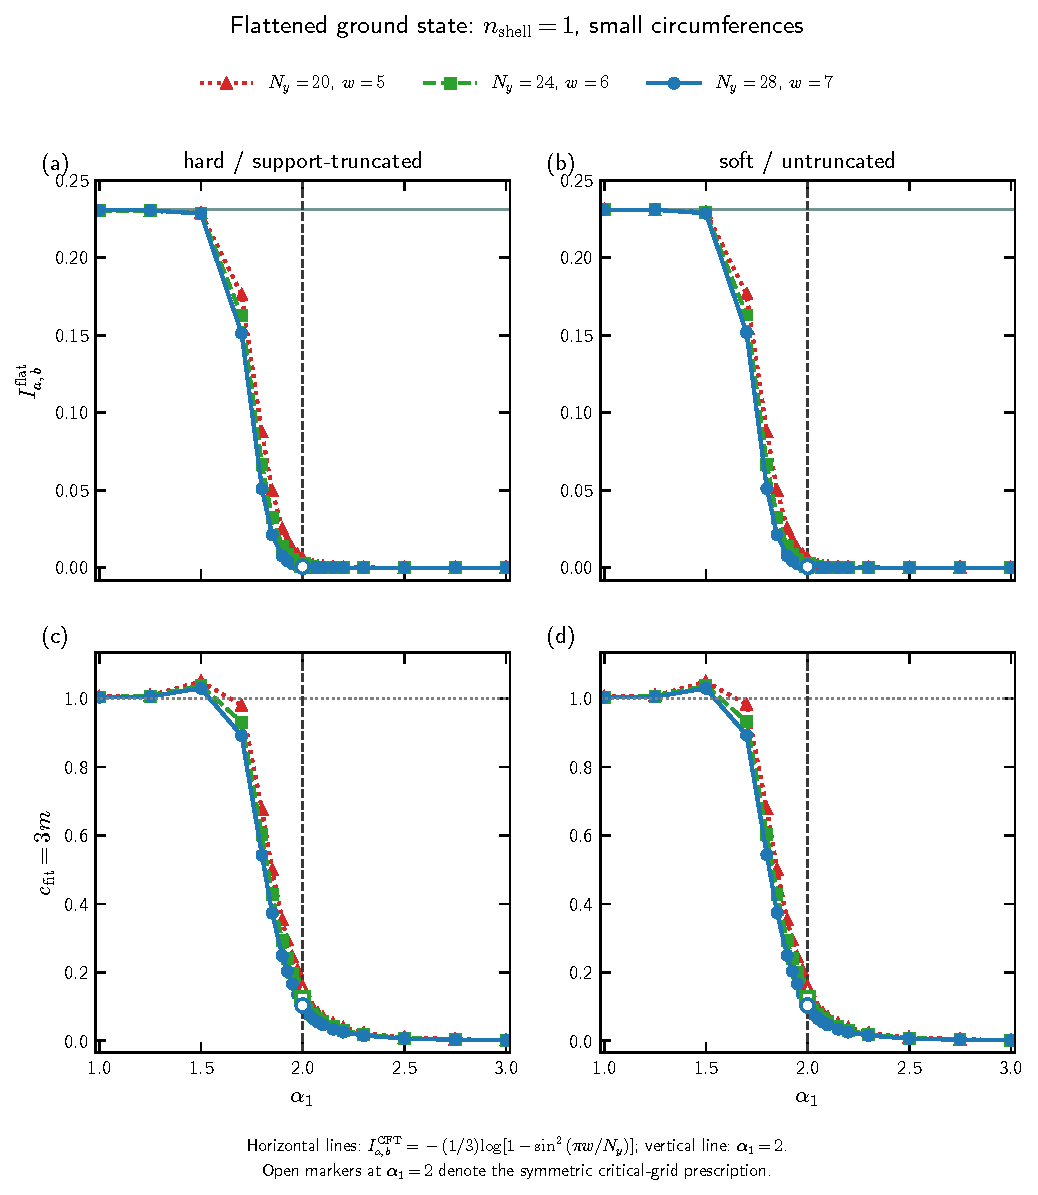
\includegraphics[width=0.99\textwidth,height=0.82\textheight,keepaspectratio]{small_ny_nshell1.pdf}
  \caption{\label{fig:small}
  Small-circumference flattened-ground-state sweep at
  $N_x=20$, $N_y=20,24,28$, $w=N_y/4=5,6,7$,
  $n_{\mathrm{shell}}=1$, and $\alpha_2=30$.  Panels (a) and (b) show
  $\Iab^{\mathrm{flat}}$ for hard/support-truncated and soft/untruncated walls;
  panels (c) and (d) show $\cfit=3m$ from
  $A_y=2,\ldots,N_y/2$.  Colored horizontal lines in the upper row are the
  $c=1$ free-Dirac references, which coincide at $(\log 2)/3$ for these exact
  quarter strips.  The gray horizontal line is $\cfit=1$, and the black dashed
  line marks $\alpha_1=2$; open markers there denote the symmetric prescription
  in Eq.~\eqref{eq:criticalprescription}.  Every curve is deterministic and has no sampling
  uncertainty; the saved regression errors are fit-residual diagnostics, not
  ensemble error bars.  Cases were evaluated on the descending grid
  $\alpha_1:3\to1$, while the display uses the conventional increasing axis.}
\end{widefigure}
\clearpage

\subsection{Large circumferences and shell dependence}

Figures~\ref{fig:large1}--\ref{fig:largeinf} separate the larger systems by
OW range so that every panel remains readable.  At $\alpha_1=1$ and
$n_{\mathrm{shell}}=1$, the exact-quarter values for $N_y=40,60$ lie between
$0.230817$ and $0.231033$; the $N_y=50$ values lie between $0.210601$ and
$0.210726$, in accord with its distinct $w=12$ reference.  The fitted central
charges are $1.0014$--$1.0023$.  Increasing to $n_{\mathrm{shell}}=2$ retains
the same mutual-information plateau and gives modest positive finite-size
curvature in $\cfit$, while moving the crossover closer to $\alpha_1=2$.

The $n_{\mathrm{shell}}=\infty$ data behave differently only in the narrow
bulk-critical region.  Just below $\alpha_1=2$, the largest observed values
are $\Iab=0.386194$ and $\cfit=1.48664$ for the hard wall at $N_y=40$ and
$\alpha_1=1.975$.  The half-filling gap at that same point is $0.176106$, and
the number of negative levels equals the imposed rank, $800$.  For the soft
wall at the same size and parameter, the gap is $0.446436$.  Thus the saved
half-filling spectrum does not show a zero-mode degeneracy at the overshoot.

The minimum gap across the campaign, $6.56\times10^{-16}$, and the only
negative-level/rank mismatch, $799$ versus $800$, instead occur for the hard
wall at $N_y=40$ and $\alpha_1=1$, where the mutual information is on its
ordinary topological plateau.  This isolated wall-mode degeneracy is not
evidence for the critical-window enhancement.  The conservative explanation
of that enhancement is that Eq.~\eqref{eq:cfit} assumes the only logarithmic
sector is the one-dimensional wall theory, whereas the two-dimensional bulk
correlation length grows rapidly near $\alpha_1=2$ and contaminates the
finite-window fit.  The overshoot is consequently a crossover diagnostic
rather than a stable $c>1$ phase.  Away from this window the large-$N_y$
curves again approach the $c=1$ plateau for $\alpha_1<2$ and zero mutual
information in the trivial regime.  Hard and soft constructions agree most
closely for finite shell and show their largest microscopic difference in the
full-frame critical window.

\section{Validation and limitations}
\label{sec:validation}

The small aggregate contains arrays of shape $(2,3,21)$ indexed by wall,
circumference, and $\alpha_1$.  The large aggregate has shape $(2,3,3,21)$,
adding the shell index.  Their completion records bind the NPZ byte counts and
SHA-256 checksums.  The manuscript renderer verifies those records before
loading any array and then checks the wall labels, sizes, widths, shell labels,
and the exact descending grid in Eq.~\eqref{eq:alphagrid}.

The final occupied-state correlation projectors satisfy stringent numerical
tests.  For the small campaign the maximum projector idempotency residual is
$2.89\times10^{-15}$ and the maximum $y$-translation residual is
$3.00\times10^{-15}$.  For the large campaign the corresponding maxima are
$5.44\times10^{-15}$ and $1.04\times10^{-14}$ for OW translation covariance.
Restricted occupation eigenvalues remain within $1.5\times10^{-14}$ of
$[0,1]$.  These checks concern the final half-filled correlation projector;
they do not turn the midpoint matrices $P_\pm(\bm0)=\mathbf{1}/2$ at
$\alpha_1=2$ into spectral projectors.  The smallest saved mutual information
is $-2.31\times10^{-12}$, a cancellation-scale roundoff value that is retained
rather than clipped; no value is negative beyond the $10^{-8}$ materiality
tolerance.

Several limitations are essential.  First, $N_x$ is fixed, so increasing
$N_y$ tests the circumference dependence of two fixed transverse domain walls
rather than isotropic two-dimensional finite-size scaling.  Second, $\cfit$
is a finite-window estimator and is not controlled when bulk modes become
critical.  Third, the exact Dirac expression for disconnected intervals does
not transfer unchanged to an interacting or otherwise generic CFT.  Fourth,
the finite periodic lattice state need not realize the conformal-vacuum spin
sector without corrections.  Finally, this ground-state reference does not
establish that the Born-weighted endpoint ensemble of the adaptive dynamics
reaches the same curve.  That comparison requires the independent trajectory
sweep, including the prescribed order of nonlinear averaging over placements
and samples.

\clearpage

\begin{widefigure}
  \centering
  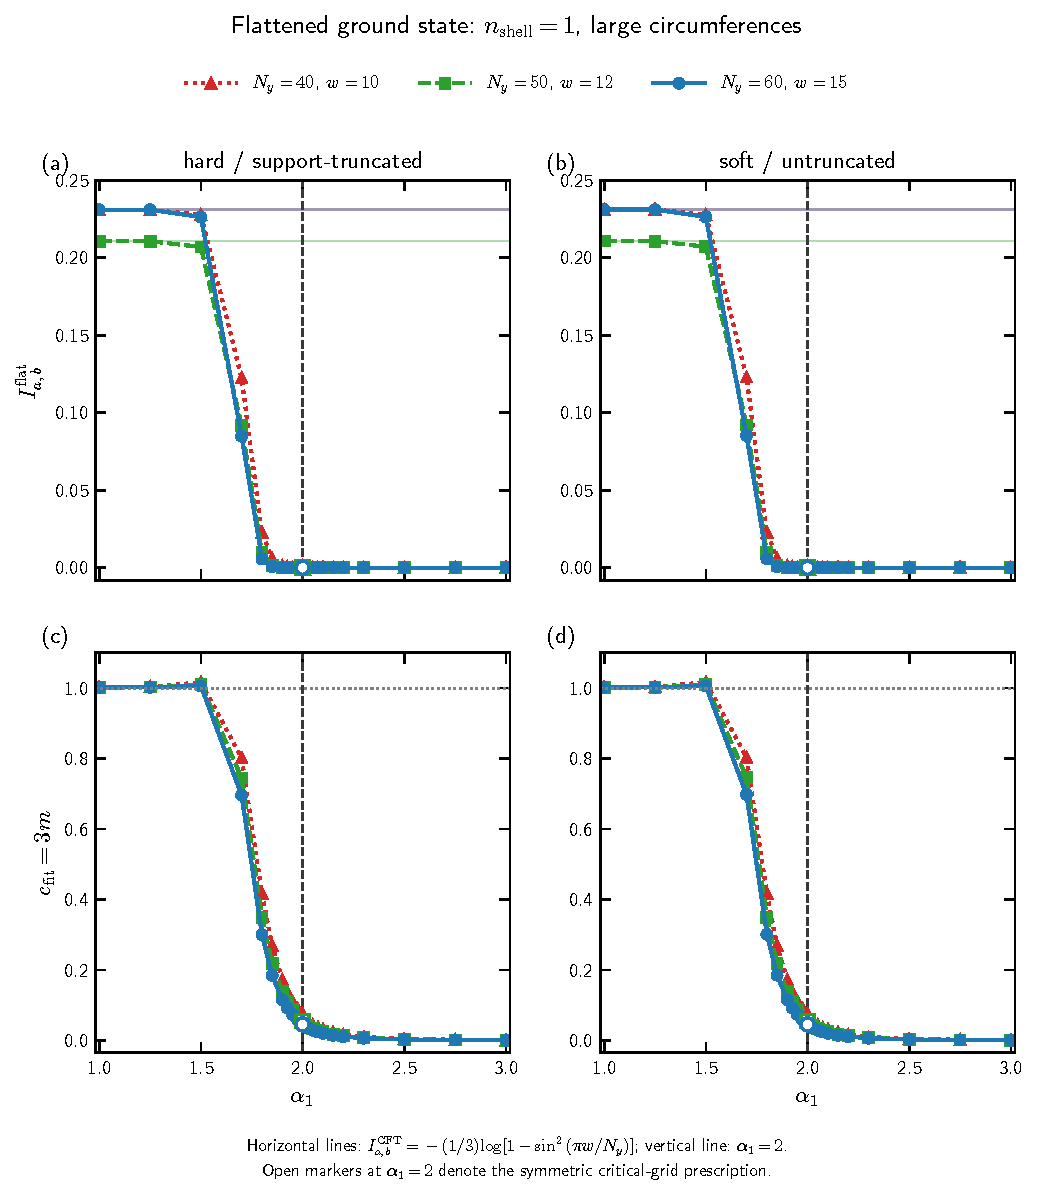
\includegraphics[width=0.99\textwidth,height=0.84\textheight,keepaspectratio]{large_ny_nshell1.pdf}
  \caption{\label{fig:large1}
  Large-circumference sweep for $n_{\mathrm{shell}}=1$ at
  $N_x=20$, $N_y=40,50,60$, $w=10,12,15$, and $\alpha_2=30$.
  Columns distinguish hard and soft walls; rows show mutual information and
  the entropy-slope estimator.  The colored reference for $N_y=50$ is
  $0.2107497$ because $w=12<50/4$; the $N_y=40,60$ references are
  $(\log 2)/3=0.2310491$.  Open markers at $\alpha_1=2$ denote the symmetric
  critical-grid prescription in Eq.~\eqref{eq:criticalprescription}; line,
  marker, fit, determinism, and sweep conventions are otherwise the same as
  Fig.~\ref{fig:small}.}
\end{widefigure}
\clearpage

\begin{widefigure}
  \centering
  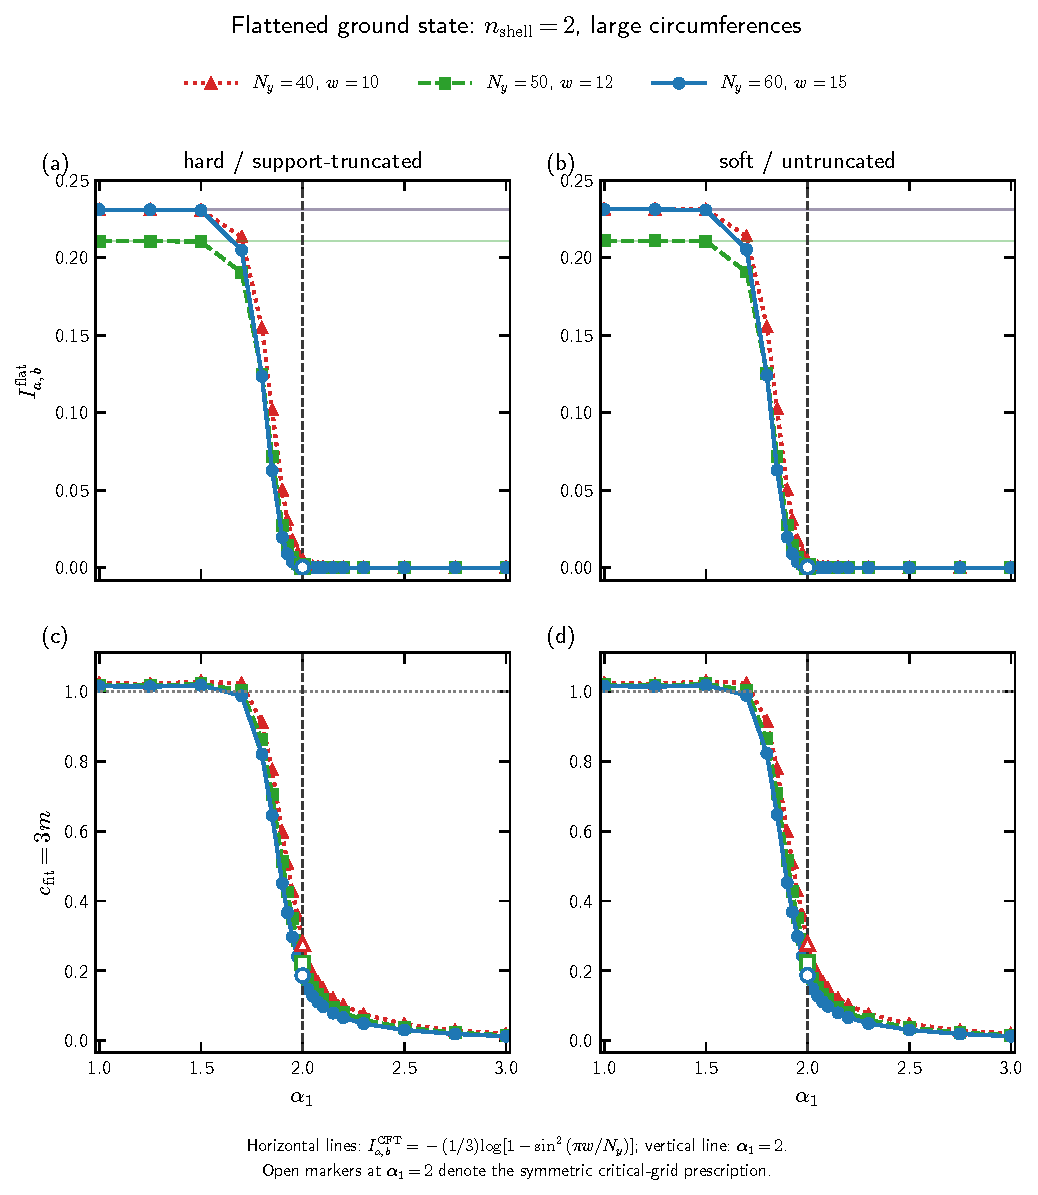
\includegraphics[width=0.99\textwidth,height=0.84\textheight,keepaspectratio]{large_ny_nshell2.pdf}
  \caption{\label{fig:large2}
  Large-circumference sweep for $n_{\mathrm{shell}}=2$, with the same geometry
  and panel organization as Fig.~\ref{fig:large1}.  Extending the OW support
  preserves the topological mutual-information plateau but shifts the rounded
  crossover toward the untruncated parent value $\alpha_1=2$.  The exact
  critical-grid points use Eq.~\eqref{eq:criticalprescription}.  No sampling
  uncertainties are present; $\cfit$ errors stored in the aggregate are
  residual errors of the chord-length regression.  Cases were evaluated from
  $\alpha_1=3$ to $1$ and are shown on an increasing horizontal axis.}
\end{widefigure}
\clearpage

\begin{widefigure}
  \centering
  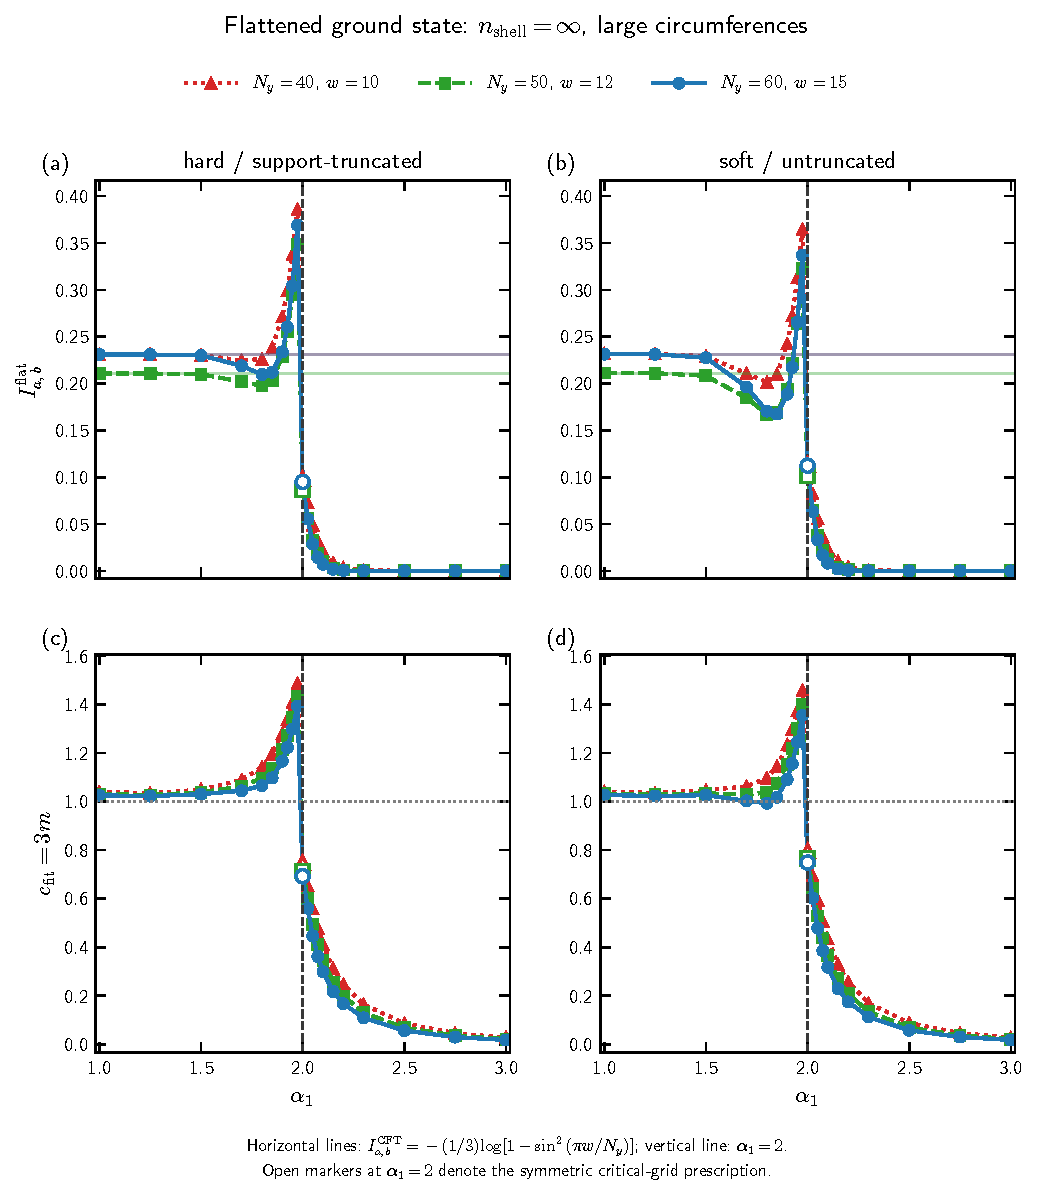
\includegraphics[width=0.99\textwidth,height=0.84\textheight,keepaspectratio]{large_ny_nshellinf.pdf}
  \caption{\label{fig:largeinf}
  Full-frame ($n_{\mathrm{shell}}=\infty$) large-circumference sweep.  The
  topological plateau at smaller $\alpha_1$ remains close to the free-Dirac
  references.  The enhancement immediately below $\alpha_1=2$ occurs where
  bulk criticality contaminates the wall-only chord fit.  The saved
  half-filling gap at the enhancement is finite; the campaign's isolated
  near-zero gap occurs instead at $\alpha_1=1$.  The enhancement is therefore
  not interpreted as a stable $c>1$ domain-wall theory or as a demonstrated
  zero-mode effect.  Hard/soft columns,
  reference lines, deterministic status, regression window, and descending
  evaluation order are as in Figs.~\ref{fig:small} and \ref{fig:large1}.}
\end{widefigure}
\clearpage

\section{Conclusion}
\label{sec:conclusion}

The flattened OW parent supplies a clean calibration of the proposed
opposite-strip observable.  In the topological regime, hard and soft walls and
all studied circumferences recover a nonzero fixed-cross-ratio mutual-
information plateau together with a single-strip entropy coefficient near
$c=1$.  The value $(\log 2)/3$ follows from the exact free-Dirac multi-interval
identity and the quarter-circle geometry, not from area-law cancellation
alone.  Its size independence is precisely what scale invariance predicts
when interval width and separation grow together.  The same derivation also
identifies the geometry needed to obtain divergent mutual information: keep a
physical gap fixed while growing the intervals, or take the adjacent-interval
limit.  These distinctions make the present curves useful quantitative
references for, but not substitutes for, the future dynamical ensemble.

\bibliographystyle{apsrev4-2}
\bibliography{references}

\end{document}
